%%% Local Variables:
%%% mode: latex
%%% TeX-master: "../main_file"
%%% End:

\section{Algorithmes de filtrage basés sur le Time-Table}
\label{sec:time_CECSP}
Le paragraphe suivant présente plusieurs algorithmes de filtrage pour le
\CECSP. Tous ces algorithmes utilisant une adaptation du Time-Table
pour le \CUSP, nous commençons donc par présenter brièvement comment
ce raisonnement est modifié pour être adapté dans le cadre du \CECSP.
Puis, nous présentons deux autres algorithmes permettant
de réduire l'ensemble des valeurs possibles pouvant être prises par
chaque variable. Le premier est adapté du Time-Table disjonctif pour
le \CUSP~\cite{Gay2015} et le dernier utilise une combinaison entre
problème de flots et profil obligatoire.

\subsection{Le Time-Table}
\label{sec:TT_CECSP}
Comme pour le \CUSP, le Time-Table pour le \CECSP~se base sur la
notion de partie obligatoire des activités, i.e. l'intervalle pendant
lequel une activité est en cours d'exécution dans tous les
ordonnancements réalisables. Cependant, comme dans le cas du \CECSP
nous ne connaissons pas la durée exacte d'une activité, nous utilisons 
une borne inférieure sur sa durée pour calculer la date de début au
plus tard, $\LS$, et la date de fin au plus tôt, $\EE$. Pour calculer
cette borne, remarquons que la configuration permettant de finir une
activité le plus rapidement possible, est celle où l'activité est
exécutée à son rendement maximal $\bmax$. De ce fait, une borne
inférieure sur la durée de l'activité vaut $W_i/f_i(\bmax)$. Nous
pouvons donc calculer la date de début au plus tard de l'activité,
$\LS=\LE -W_i/f_i(\bmax)$, et sa date de fin au plus tôt,
$\EE=\ES +W_i/f_i(\bmax)$. La partie obligatoire d'une activité $i$ est
alors définie de la même manière que pour le \CUSP, i.e la partie
obligatoire de $i$ est l'intervalle $[\LS,\EE{[}$
(cf. figure~\ref{fig_mand_CECSP}).

Cependant, dans le cas où $\LS \le \EE$, i.e. où l'activité possède
une partie obligatoire, nous pouvons seulement déduire que l'activité
$i$ va consommer au moins une quantité $\bmin$ de la ressource durant
toute sa partie obligatoire, et ce, quel que soit le moment où
l'activité est ordonnancée. La notion de profil obligatoire de la
ressource est donc légèrement différente de celle définie pour le
\CUSP~(cf. définition~\ref{def:profil_oblig},
page~\pageref{def:profil_oblig}).

\begin{defi}
Le profil obligatoire d'une ressource $TT_{\A}$ dans le cas du
\CECSP~est défini de la façon suivante: 
\[TT_{\A}(t)=\sum_{\substack{i \in \A\\\LS \le t \le \EE}} \bmin\quad
  \forall t \in \H\]
Le problème est donc insatisfiable dans le cas où $\exists t \in \H\
:\ TT_{\A}(t) > R$
\end{defi}

\begin{ex}
Considérons l'activité suivante: 

\vspace{-0.5cm}
\begin{center}
  \begin{tabular}{|P{1cm}P{1cm}P{1cm}P{1cm}P{1cm}P{2cm}|}
    \hline
    \ES & \LE & W_i & \bmin & \bmax & f_i(b_i(t))\\
    \hline
    1 & 14 & 72 & 2 & 5 & b_i(t)+3\\
    \hline
  \end{tabular}
\end{center}

Nous pouvons calculer sa date de début au plus tard,
$\LS=\LE -W_i/f_i(\bmax)=14 - 72/8 =5$, ainsi que sa date de fin au
plus tôt, $\EE=\ES + W_i/f_i(\bmax)=1 + 72/8 =10$. Comme $\EE > \LS$,
l'activité possède une partie obligatoire qui est l'intervalle
$[5,10[$ (voir
figure~\ref{fig_mand_CECSP_a},~\ref{fig_mand_CECSP_b}). Cependant,
nous pouvons seulement en déduire que l'activité sera en cours dans
cet intervalle et, grâce à la borne inférieure sur la quantité de
ressource que peut consommer l'activité durant son exécution, nous
pouvons déduire que, sur l'intervalle $[\LS,\EE{[}=[5,10[$, l'activité est au
moins exécutée à $\bmin$ (voir figure~\ref{fig_mand_CECSP_c}).
  
\begin{figure}[htb!]
\vspace{-0.8cm}
\subcaptionbox{Ordonnancement au plus tôt\label{fig_mand_CECSP_a}}[0.3\linewidth]{
    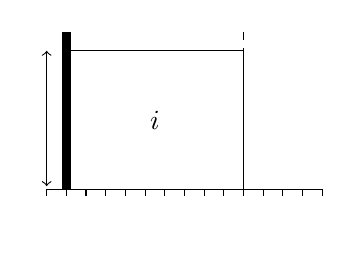
\begin{tikzpicture}
      [xscale=0.25, yscale= 0.4,node distance=0.5cm]
      \node (sil) at (1,0) {} ;
      \node (eil) at (10,0) {} ;
      \node [below of=eil,node distance=0.63cm]  {$\EE$};
      \draw (sil.center) node[below=0.2cm] {$\ES$};
      
      \draw (0,0) -- (14,0);
      \draw[line width=3pt] (1,0) -- (1,5);
      
      \draw[<->] (0,0.1) -- (0,4.4) node[midway,left] {$\bmax$};
      \draw (1,0) rectangle (10,4.4) node[midway] {$i$};

      \draw[dashed] (10,0) -- (10,5);

      \foreach \i in {0,...,14} {
        \draw (\i,0)  -- (\i,-0.2);
      }
    \end{tikzpicture}
}
\hfill
\subcaptionbox{Ordonnancement au plus tard\label{fig_mand_CECSP_b}}[0.3\linewidth]{
    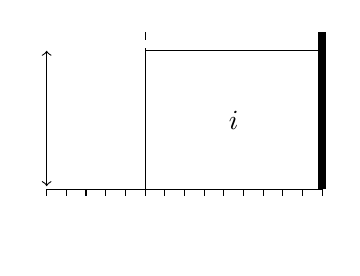
\begin{tikzpicture}
      [xscale=0.25, yscale= 0.4,node distance=0.5cm]
      \node (sir) at (5,0) {} ;
      \node (eir) at (14,0) {} ;
      \node[below of= sir,node distance=0.63cm] {$\LS$};
      \draw (eir.center) node[below=0.2cm] {$\LE$};
      
      \draw (0,0) -- (14,0);
      \draw[line width=3pt] (14,0) -- (14,5);
      
      \draw[<->] (0,0.1) -- (0,4.4) node[midway,left] {$\bmax$};
      \draw (5,0) rectangle (14,4.4) node[midway] {$i$};

      \draw[dashed] (5,0) -- (5,5);

      \foreach \i in {0,...,14} {
        \draw (\i,0)  -- (\i,-0.2);
      }
    \end{tikzpicture}
}
\hfill
\subcaptionbox{Ordonnancement réalisable à $\bmin$ dans
  $[\LS,\EE]$ \label{fig_mand_CECSP_c}}[0.3\linewidth]{ 
    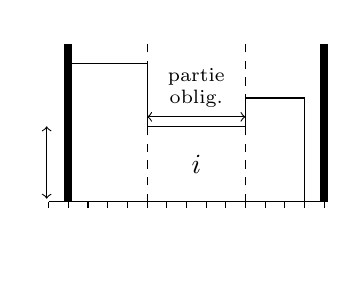
\begin{tikzpicture}
      [xscale=0.25, yscale= 0.4,node distance=0.5cm]
      \node (sir) at (5,0) {} ;
      \node (eil) at (10,0) {} ;
      \node [below of=eil,node distance=0.63cm]  {$\EE$};
      \node[below of= sir,node distance=0.63cm] {$\LS$};
      \draw[<->] (5,2.7) -- (10,2.7) node[midway,above,text width=1.4cm]
      {\begin{center} \scriptsize partie oblig. \end{center}};
      
      \draw[white] (5,0) rectangle (10,2.4) node[midway,color=black] {$i$};
           
      \draw (1,4.4) -- (5,4.4) -- (5,2.4) -- (10,2.4) -- (10,3.3) --
      (13,3.3) -- (13,0);
      
      \draw (0,0) -- (14,0);
      \draw[line width=3pt] (1,0) -- (1,5);
      \draw[line width=3pt] (14,0) -- (14,5);
      
      \draw[<->] (-0.1,0.1) -- (-0.1,2.4) node[midway,left] {$\bmin$};
    


      \draw[dashed] (5,0) -- (5,5);
      \draw[dashed] (10,0) -- (10,5);

      \foreach \i in {0,...,14} {
        \draw (\i,0)  -- (\i,-0.2);
      }
    \end{tikzpicture}
}
\caption{Partie obligatoire d'une activité $i$ pour le \CECSP.}
\label{fig_mand_CECSP}
\end{figure}
\end{ex}

Comme pour la contrainte cumulative, le profil obligatoire peut aussi
être calculé en $O(n)$ à l'aide d'un algorithme de balayage en triant
au préalable les activités par date de début au plus tard et date de
fin au plus tôt.

Nous détaillons maintenant l'adaptation du Time-Table disjonctif au
\CECSP. 

\subsection{Le Time-Table disjonctif}
\label{sec:TTDR_CECSP}

Le second algorithme de filtrage proposé repose sur un raisonnement
appelé Time-Table disjonctif et utilisé, en premier lieu, pour le
\CUSP~(cf. paragraphe~\ref{sec:mix_CUSP}). Ce dernier repose sur le
raisonnement Time-Table décrit précédemment et sur le raisonnement
disjonctif.

Le raisonnement disjonctif dans le cadre du \CECSP~est très similaire
à celui défini pour le \CUSP. La différence repose sur la construction
des ensembles disjonctifs. Dans le cas du \CECSP, un couple
d'activités ($i,j)$ sera dit disjonctif si $\bmin+\bmin[j] >R$. Dans
ce cas, nous savons que:
\begin{itemize}
\item l'activité $i$ doit commencer après l'activité $j$, ou 
\item l'activité $i$ doit finir avant l'activité $j$.  
\end{itemize}

Cette propriété permet notamment d'ajuster la date de début au
plus tôt de d'une des deux activités. Considérons par exemple le cas
où $\ES[j] \le \EE$ et $\LS < \EE[j]$; ces relations 
impliquent que $j$ doit commencer après la fin de l'activité $i$ (voir
figure~\ref{fig:disj_CECSP}). De ce fait, le début de $j$ ne peut
arriver avant la date de fin au plus tôt de $i$, et donc: $\ES[j] \ge
\EE$. La règle de filtrage est ensuite similaire à celle mise en place
pour le \CUSP.

\begin{reg}
Soient $i, j \in \A, i \neq j$ telles que $\bmin+\bmin[j] < R$ et $\LS
< \EE[j]$. Alors la date de début au plus tôt de l’activité peut être
ajustée et on a : $\ES[j] \ge \EE$.
\end{reg}

\begin{ex}
Considérons l'instance à deux activités et avec une ressource de
capacité $3$ suivante: 
\begin{center}
\begin{tabular}{|P{1cm}|P{1cm}P{1cm}P{1cm}P{1cm}P{1cm}P{2cm}|}
    \hline
    act & \ES & \LE & W_i & \bmin & \bmax & f_i(b_i(t))  \\
    \hline
   i & 2 & 11 & 28 & 2 & 3 & 2*b_i(t) +1\\
   j & 1 & 20 & 49 & 2 & 4 & voir fig.~\ref{fig:fonct_CECSP}\\
    \hline
  \end{tabular}
\end{center}

La fonction $f_j(b_j(t))$ est définie par l'expression suivante: 
\[f_j(b_j(t))=\left\{
\begin{array}{lll}
2b_j(t) & & b_j(t) \in [2,3]\\
b_j(t)+3 & & b_j(t) \in [3,4]
\end{array}
\right.\] 
et décrite dans la figure~\ref{fig:fonct_CECSP}
\begin{figure}[!htb]
\centering
\begin{tikzpicture}
[xscale=0.8,yscale=0.56]
\node (O) at (1,2) {};
\draw[->] (1,2) -- (5.5,2);
\draw[->] (1,2) -- (1,8);

\path[draw] (2,4) -- (3,6) -- (4,7) ;

\draw[dotted] (2,2) node[below] {\footnotesize $2$} -- (2,8);
\draw[dotted,color=gray!70] (4,2) node[below,color=black] {\footnotesize $4$}
-- (4,8);
\draw[dotted] (3,2) node[below] {\footnotesize $3$} -- (3,8);

\draw (1,4) node[left] {\footnotesize $4$};
\draw (1,6) node[left] {\footnotesize $6$};
\draw (1,7) node[left] {\footnotesize $7$};
\end{tikzpicture}
\caption{Fonction $f_j(b_j(t))$.}
\label{fig:fonct_CECSP}
\end{figure}

Dans cet exemple, comme $\bmin +\bmin[j] =4 > 3$, $i$ et $j$ ne
peuvent s'exécuter en parallèle. Si l'activité $i$ finit au temps
$\LE= 11$ alors, elle chevauche forcément l'activité $j $ (voir
figure~\ref{fig:disj_CECSPa} et~\ref{fig:disj_CECSPb}). Dans tout
ordonnancement réalisable, $i$ est donc exécutée avant $j$ et la date de
début au plus tôt de $j$ peut donc être ajustée, i.e. $j$ ne peut
commencer avant $\EE=6$ (voir
figure~\ref{fig:disj_CECSPc}).
  \begin{figure}[htb!] 
    \subcaptionbox{Si $i$ finit au temps $11$...\label{fig:disj_CECSPa}}[0.45\linewidth]{
    \centering
    \begin{tikzpicture} [yscale=0.4,xscale=0.4]   
        \node (O) at (0,0) {};
      \foreach \i in {0,5,...,10} {
        \draw (\i,0) -- (\i,-0.1) node[below] {\small $\i$};
      }
      \fill[gray!50] (2,0) rectangle (11,3.4);
      \fill[gray!50] (1,3.6) rectangle (14,8);
      
      \draw[fill=white] (6.4,0.2) -- (6.4,3.2)   -- (8.4,3.2) -- (8.4,2) --node[midway,below=0.2cm] {$i$}
      (11,2) -- (11,0.2) -- cycle;
      
      \draw[fill=white] (1,3.8) -- (1,7.8)  node[midway,right=0.6cm] {$j$} -- (6,7.8) -- (6,5.8) --
      (9.5,5.8) -- (9.5,3.8) -- cycle;
      \draw[white, pattern=north west lines] (6.4,0) rectangle (9.5,8);

      \draw[->] (0,0) -- (14,0);
      \draw[->] (0,0) -- (0,8) ;
      \draw (0,3) node[left] {$R=3$};
      \draw[densely dotted] (1,-0.1) -- (1,8) node[above] {$\ES[j]$};
      \draw[densely dotted] (8,-0.1) -- (8,8) node[above] {$\EE[j]$};
      \draw[densely dotted] (2,-0.1)  node[below] {$\ES$}-- (2,8);
      \draw[densely dotted] (6,-0.1 ) node[below=0.4cm] {$\EE$}-- (6,8) ;
      \draw[densely dotted] (7,-0.1) node[below] {$\LS$} -- (7,8) ;
      \draw[densely dotted] (11,-0.1) node[below right] {$\LE$} -- (11,8) ;
      \draw[<->] (14.5,0.2) -- (14.5,3.2) node[midway,right] {$\bmax$} ;
      \draw[<->] (14.5,3.8) -- (14.5,7.8) node[midway,right] {$\bmax[j]$} ;   
    \end{tikzpicture}
  }
    \subcaptionbox{...alors $i$ chevauche forcément l'activité $j$\label{fig:disj_CECSPb}}[0.45\linewidth]{
        \centering
        \begin{tikzpicture}[yscale=0.4,xscale=0.4]
      \node (O) at (0,0) {};
      \foreach \i in {0,5,...,10} {
        \draw (\i,0) -- (\i,-0.1) node[below] {\small $\i$};
      }
      \fill[gray!50] (2,0) rectangle (11,3.4);
      \fill[gray!50] (1,3.6) rectangle (14,8);
      
      \draw[fill=white] (7,0.2) rectangle (11,3.2) node[midway]
      {$i$};
      \draw[fill=white] (1,3.8) rectangle (8,7.8) node[midway]
      {$j$};
      \draw[white, pattern=north west lines] (7,0) rectangle (8,8);

      \draw[->] (0,0) -- (14,0);
      \draw[->] (0,0) -- (0,8) ;
      \draw (0,3) node[left] {$R=3$};
      \draw[densely dotted] (1,-0.1) -- (1,8) node[above] {$\ES[j]$};
      \draw[densely dotted] (8,-0.1) -- (8,8) node[above] {$\EE[j]$};
      \draw[densely dotted] (2,-0.1)  node[below] {$\ES$}-- (2,8);
      \draw[densely dotted] (6,-0.1 ) node[below=0.4cm] {$\EE$}-- (6,8) ;
      \draw[densely dotted] (7,-0.1) node[below] {$\LS$} -- (7,8) ;
      \draw[densely dotted] (11,-0.1) node[below right] {$\LE$} -- (11,8) ;
      % \draw[densely dotted] (6,-0.1) -- (6,8) node[above] {$\ES[j]^{'}$};
      % \draw[->] (1.8,5.8) -- (5.2,5.8);
      \draw[<->] (14.5,0.2) -- (14.5,3.2) node[midway,right] {$\bmax$} ;
      \draw[<->] (14.5,3.8) -- (14.5,7.8) node[midway,right]
      {$\bmax[j]$} ;
    \end{tikzpicture}
   }
    \subcaptionbox{$\ES[j]$ peut être ajusté\label{fig:disj_CECSPc}}[\linewidth]{    \centering
      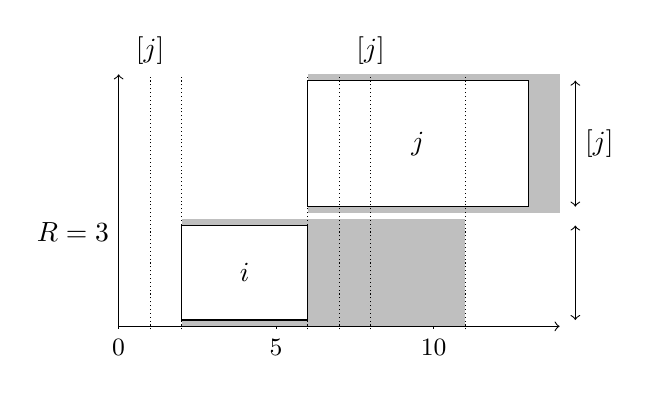
\begin{tikzpicture} [yscale=0.4,xscale=0.4]
      \node (O) at (0,0) {};
      \foreach \i in {0,5,...,10} {
        \draw (\i,0) -- (\i,-0.1) node[below] {\small $\i$};
      }
      \fill[gray!50] (2,0) rectangle (11,3.4);
      \fill[gray!50] (6,3.6) rectangle (14,8);
      
      \draw[fill=white] (2,0.2) rectangle (6,3.2) node[midway]
      {$i$};
      \draw[fill=white] (6,3.8) rectangle (13,7.8) node[midway]
      {$j$};

      \draw[->] (0,0) -- (14,0);
      \draw[->] (0,0) -- (0,8) ;
      \draw (0,3) node[left] {$R=3$};
      \draw[densely dotted] (1,-0.1) -- (1,8) node[above] {$\ES[j]$};
      \draw[densely dotted] (8,-0.1) -- (8,8) node[above] {$\EE[j]$};
      \draw[densely dotted] (2,-0.1)  node[below] {$\ES$}-- (2,8);
      \draw[densely dotted] (6,-0.1 ) node[below=0.4cm] {$\EE$}-- (6,8) ;
      \draw[densely dotted] (7,-0.1) node[below] {$\LS$} -- (7,8) ;
      \draw[densely dotted] (11,-0.1) node[below right] {$\LE$} -- (11,8) ;
      \draw[<->] (14.5,0.2) -- (14.5,3.2) node[midway,right] {$\bmax$} ;
      \draw[<->] (14.5,3.8) -- (14.5,7.8) node[midway,right] {$\bmax[j]$} ;

  \end{tikzpicture}
}
  \caption{Raisonnement disjonctif pour le \CECSP.}
  \label{fig:disj_CECSP}
\end{figure}
\end{ex}

Nous pouvons maintenant présenter l'adaptation du Time-Table
disjonctif au cas du \CECSP. Pour ce faire, nous commençons par
adapter la définition d'intervalle minimum de superposition, puis nous
présenterons les modifications apportées aux règles d'ajustement du
\CUSP~afin que ces dernières soient applicables dans le cas du
\CECSP.

La notion d'intervalle minimum de superposition est légèrement plus
difficile à définir que dans le cas du \CUSP. En effet, cet intervalle
représente l'ensemble minimal de points de temps tel qu'une activité
$i$ est forcément en cours durant un de ces points et, comme au point
$\EE$, l'activité n'est pas forcément en cours, il faut inclure le
point ``juste à gauche'' de $\EE$ dans $moi_i$.  La définition peut
donc s'écrire de la manière suivante. 

\begin{defi}
\label{des:moi_CUSP} 
Soit $\EE^{-}$ le point le plus proche de $\EE > 0$, i.e. $\forall \delta
>0 , |\EE^{-} -\EE| \le \delta$. L'intervalle minimum de
superposition d'une activité $i$,noté $moi_i$, est alors défini par
$moi_i=[\EE^{-},\LS{]}$ si $i$ ne possède pas de partie obligatoire et
$moi_i=\emptyset$ sinon.   
\end{defi}

\begin{ex}
La figure~\ref{fig:moi_CECSP} illustre l'intervalle minimum de
superposition d'une activité $i$ ne possédant pas de partie
obligatoire. En effet, quelle que soit la position de l'activité $i$,
elle intersecte forcément $moi_i$.
\begin{figure}[!htb]
  \begin{center}
    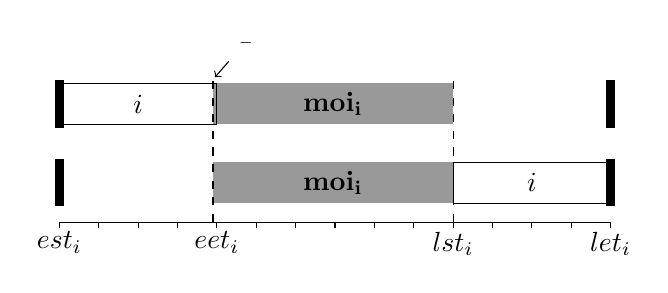
\begin{tikzpicture}
      [xscale=0.5, yscale= 0.4,node distance=0.5cm][decoration={brace}]
      \node (sil) at (0,0) {} ;
      \node (sir) at (10,0) {}; 
      \draw (10,0) node[below] {$lst_i$};
      \node (eir) at (14,0) {} ;
      \node (eil) at (4,0) {} ;
      \draw (4,0) node [below]  {$eet_i$} ;
      \draw (sil.center) node[below] {$est_i$}--
      (eir.center) node[below] {$let_i$};
      
      \draw[<-] (3.95, 4.6) -- (4.3,5.1) node[above=0.2cm,right] {\scriptsize $\EE^{-}$};
      \draw[line width=3pt] (0,0.5) -- (0,2);
      \draw[line width=3pt] (14,0.5) -- (14,2);
      \draw[line width=3pt] (0,3) -- (0,4.5);
      \draw[line width=3pt] (14,3) -- (14,4.5);

      \fill[gray!80] (3.9,0.6) rectangle (10,1.9) node[midway,color=black] {$\mathbf{moi_i}$};
      \fill[gray!80] (3.9,3.1) rectangle (10,4.4) node[midway,color=black] {$\mathbf{moi_i}$};
      
      \draw (0,3.1) rectangle (4,4.4) node[midway] {$i$};
      \draw (10,0.6) rectangle (14,1.9) node[midway] {$i$};

      \draw[dashed] (3.9,0) -- (3.9,4.5);
      \draw[dashed] (10,0) -- (10,4.5);

      \foreach \i in {0,...,14} {
        \draw (\i,0)  -- (\i,-0.2);
      }
    \end{tikzpicture}
  \end{center}

  \caption{Intervalle minimum de superposition d'une activité dans le
    cadre du \CECSP.}
  \label{fig:moi_CECSP}
\end{figure}
\end{ex}

Cependant, pour s'abstraire du point $\EE^{-}$ et faciliter les
notations, nous n'utiliserons pas cet intervalle pour définir les
règles d'ajustement mais, à la place, nous les écrirons à l'aide
d'inégalité stricte. Ces intervalles apparaîtront cependant sur les
figures illustrant ces règles afin de faciliter leur compréhension et
de les rapprocher de celles définies pour le \CUSP.

Pour améliorer le raisonnement disjonctif, nous utilisons l'idée
suivante: si deux activités $i$ et $j$ ne peuvent être exécutées en
parallèle, alors la fenêtre de temps de $j$ ne peut contenir un point
de temps que $i$ devra forcément chevaucher. Ceci nous permet de
définir la règle d'ajustement suivante:   

\begin{reg}
\label{reg:RDR_CECSP}
  Soient deux activités $i$ et $j$ telles que $i$ ne possède pas de
  partie obligatoire et $\bmin + \bmin[j] > R$. Si $\ES[j] < \EE$ et $
  \EE[j] \le \LS$ alors $\ES[j] \ge \EE$.
\end{reg}

\begin{ex}
Considérons l'instance à deux activités et avec une ressource de
capacité $3$ suivante: 
\begin{center}
\begin{tabular}{|P{1cm}|P{1cm}P{1cm}P{1cm}P{1cm}P{1cm}P{2cm}|}
    \hline
    act & \ES & \LE & W_i & \bmin & \bmax & f_i(b_i(t))  \\
    \hline
   i & 0 & 14 & 28 & 2 & 3 & 2*b_i(t) +1\\
   j & 2 & 20 & 49 & 2 & 4 & voir fig.~\ref{fig:fonct_CECSP}\\
    \hline
  \end{tabular}
\end{center}


La règle~\ref{reg:RDR_CECSP} est illustrée par la
figure~\ref{fig:RDR_CECSP}. Dans les figures~\ref{fig:RDR_CECSPa}
et~\ref{fig:RDR_CECSPb}, on peut constater que si l'activité $j$
commence à $\ES[j]$, alors elle intersecterait complètement $moi_i$ et
il serait impossible d'ordonnancer $i$. Sur la
figure~\ref{fig:RDR_CECSPc}, $\ES[j]$ a été ajusté et l'activité $j$
ne peut commencer avant $\EE$.
  \begin{figure}[htb!] 
    \subcaptionbox{Si $j$ commence au temps $2$...\label{fig:RDR_CECSPa}}[0.45\linewidth]{
    \centering
    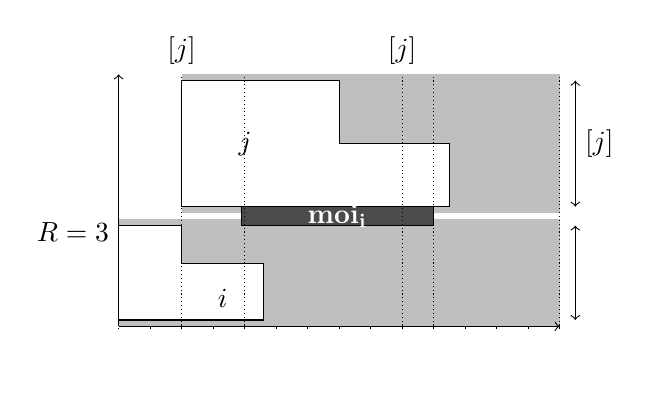
\begin{tikzpicture} [yscale=0.4,xscale=0.4]   
        \node (O) at (0,0) {};
      \foreach \i in {1,...,14} {
        \draw (\i,0) -- (\i,-0.1) ;
      }
      \fill[gray!50] (0,0) rectangle (14,3.4);
      \fill[gray!50] (2,3.6) rectangle (14,8);
      
      \draw[fill=white] (0,0.2) -- (0,3.2)   -- (2,3.2) -- (2,2) --node[midway,below=0.2cm] {$i$}
      (4.6,2) -- (4.6,0.2) -- cycle;
      
      \draw[fill=white] (2,3.8) -- (2,7.8)  node[midway,right=0.6cm] {$j$} -- (7,7.8) -- (7,5.8) --
      (10.5,5.8) -- (10.5,3.8) -- cycle;

        \draw[fill=black!70!] (3.9,3.2) rectangle
        (10,3.8) node[midway,white] {$\mathbf{moi_i}$};

      \draw[->] (0,0) -- (14,0);
      \draw[->] (0,0) -- (0,8) ;
      \draw (0,3) node[left] {$R=3$};
      \draw[densely dotted] (2,-0.1) -- (2,8) node[above] {$\ES[j]$};
      \draw[densely dotted] (9,-0.1) -- (9,8) node[above] {$\EE[j]$};
      \draw[densely dotted] (0,-0.1)  node[below] {$\ES$}-- (0,8);
      \draw[densely dotted] (4,-0.1 ) node[below=0.4cm] {$\EE$}-- (4,8) ;
      \draw[densely dotted] (10,-0.1) node[below] {$\LS$} -- (10,8) ;
      \draw[densely dotted] (14,-0.1) node[below right] {$\LE$} -- (14,8) ;
      \draw[<->] (14.5,0.2) -- (14.5,3.2) node[midway,right] {$\bmax$} ;
      \draw[<->] (14.5,3.8) -- (14.5,7.8) node[midway,right] {$\bmax[j]$} ;   
    \end{tikzpicture}
  }
    \subcaptionbox{...alors $j$ chevauche forcément $moi_i$\label{fig:RDR_CECSPb}}[0.45\linewidth]{
        \centering
        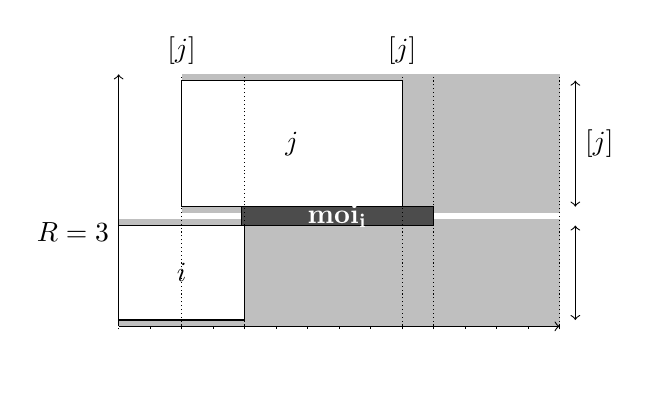
\begin{tikzpicture}[yscale=0.4,xscale=0.4]
      \node (O) at (0,0) {};
      \foreach \i in {1,...,14} {
        \draw (\i,0) -- (\i,-0.1) ;
      }
      \fill[gray!50] (0,0) rectangle (14,3.4);
      \fill[gray!50] (2,3.6) rectangle (14,8);
      
      \draw[fill=white] (0,0.2) rectangle (4,3.2) node[midway]
      {$i$};
      \draw[fill=white] (2,3.8) rectangle (9,7.8) node[midway]
      {$j$}; 
      \draw[fill=black!70!] (3.9,3.2) rectangle
        (10,3.8) node[midway,white] {$\mathbf{moi_i}$};

      
      \draw[->] (0,0) -- (14,0);
      \draw[->] (0,0) -- (0,8) ;
      \draw (0,3) node[left] {$R=3$};
      \draw[densely dotted] (2,-0.1) -- (2,8) node[above] {$\ES[j]$};
      \draw[densely dotted] (9,-0.1) -- (9,8) node[above] {$\EE[j]$};
      \draw[densely dotted] (0,-0.1)  node[below] {$\ES$}-- (0,8);
      \draw[densely dotted] (4,-0.1 ) node[below=0.4cm] {$\EE$}-- (4,8) ;
      \draw[densely dotted] (10,-0.1) node[below] {$\LS$} -- (10,8) ;
      \draw[densely dotted] (14,-0.1) node[below right] {$\LE$} -- (14,8) ;
      % \draw[densely dotted] (6,-0.1) -- (6,8) node[above] {$\ES[j]^{'}$};
      % \draw[->] (1.8,5.8) -- (5.2,5.8);
      \draw[<->] (14.5,0.2) -- (14.5,3.2) node[midway,right] {$\bmax$} ;
      \draw[<->] (14.5,3.8) -- (14.5,7.8) node[midway,right]
      {$\bmax[j]$} ;
    \end{tikzpicture}
   }
    \subcaptionbox{$\ES[j]$ peut être ajusté\label{fig:RDR_CECSPc}}[\linewidth]{    \centering
      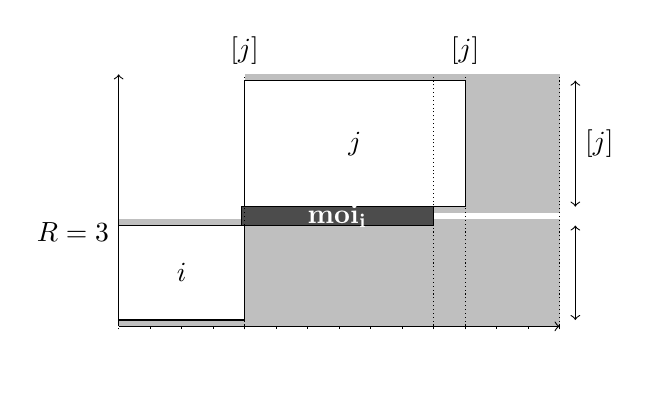
\begin{tikzpicture} [yscale=0.4,xscale=0.4]
      \node (O) at (0,0) {};
      \foreach \i in {1,...,14} {
        \draw (\i,0) -- (\i,-0.1);
      }
      \fill[gray!50] (0,0) rectangle (14,3.4);
      \fill[gray!50] (4,3.6) rectangle (14,8);
      
      \draw[fill=white] (0,0.2) rectangle (4,3.2) node[midway]
      {$i$};
      \draw[fill=white] (4,3.8) rectangle (11,7.8) node[midway]
      {$j$};
      \draw[fill=black!70!] (3.9,3.2) rectangle
        (10,3.8) node[midway,white] {$\mathbf{moi_i}$};

      \draw[->] (0,0) -- (14,0);
      \draw[->] (0,0) -- (0,8) ;
      \draw (0,3) node[left] {$R=3$};
      \draw[densely dotted] (4,-0.1) -- (4,8) node[above] {$\ES[j]$};
      \draw[densely dotted] (11,-0.1) -- (11,8) node[above] {$\EE[j]$};
      \draw[densely dotted] (0,-0.1)  node[below] {$\ES$}-- (0,8);
      \draw[densely dotted] (4,-0.1 ) node[below=0.4cm] {$\EE$}-- (4,8) ;
      \draw[densely dotted] (10,-0.1) node[below] {$\LS$} -- (10,8) ;
      \draw[densely dotted] (14,-0.1) node[below right] {$\LE$} --
      (14,8) ;
      \draw[<->] (14.5,0.2) -- (14.5,3.2) node[midway,right] {$\bmax$} ;
      \draw[<->] (14.5,3.8) -- (14.5,7.8) node[midway,right] {$\bmax[j]$} ;

  \end{tikzpicture}
}
  \caption{Raisonnement disjonctif restreint pour le \CECSP.}
  \label{fig:RDR_CECSP}
\end{figure}
\end{ex}

La règle~\ref{reg:RDR_CECSP} compare seulement les consommations de $i$
et de $j$ avec la capacité de la ressource $R$. Cependant, les
consommations obligatoires des autres activités peuvent ne pas laisser
$R$ unités de ressource durant l'intersection de $i$ et de $j$. La
règle suivante prend donc en considération le profil obligatoire de la
ressource. 

\begin{reg}
\label{reg:TTDR_CECSP}
Soient $i$ et $j$ deux activités qui ne possèdent pas de partie
obligatoire et telles que $ \bmin +\bmin[j] + \min_{\EE \le t \le \LS}
TT_{\A}(t) > R$. Si $\ES[j] < \EE$ et $ \EE[j] \le \LS$ alors $\ES[j]
\ge \EE$.
\end{reg}

\begin{ex}
Considérons l'instance à deux activités et avec une ressource de
capacité $3$ suivante: 
\begin{center}
\begin{tabular}{|P{1cm}|P{1cm}P{1cm}P{1cm}P{1cm}P{1cm}P{2cm}|}
    \hline
    act & \ES & \LE & W_i & \bmin & \bmax & f_i(b_i(t))  \\
    \hline
   i & 2 & 11 & 21 & 1 & 2 & 2*b_i(t) +1\\
   j & 1 & 20 & 14 & 1 & 2 & b_i(t)\\
   k & 2 & 11 & 18 & 2 & 2 & \frac{1}{3}*b_i(t) + \frac{4}{3}\\
    \hline
  \end{tabular}
\end{center}


  Les activités $1$ et $2$ ne possèdent pas de partie obligatoire tandis
  que l'activité $3$ est forcément en cours d'exécution durant
  l'intervalle $[2,11[$. 


  \begin{figure}[!htb]
    \centering
    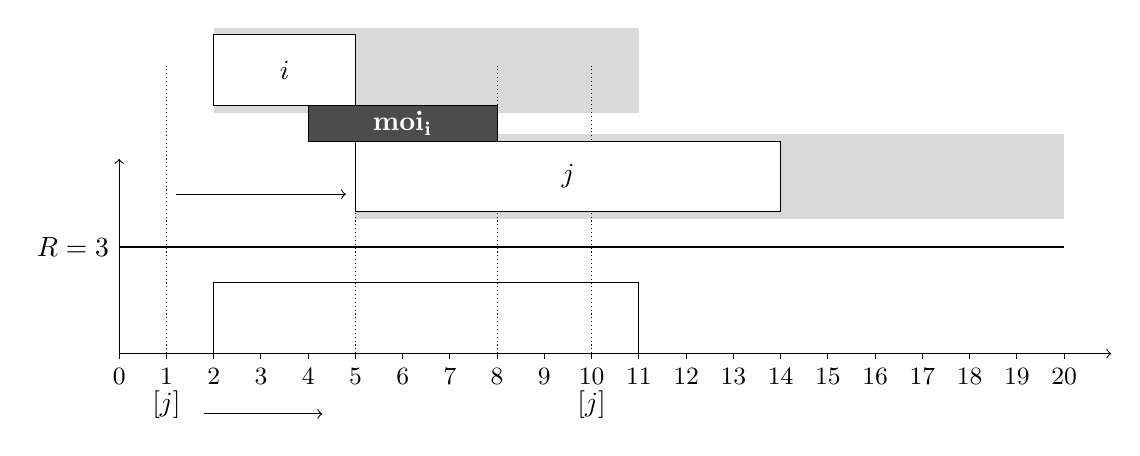
\begin{tikzpicture}
      [yscale=0.45,xscale=0.6]
      \node (O) at (0,0) {};
      \foreach \i in {0,1,...,20} {
        \draw (\i,0) -- (\i,-0.15) node[below] {\small $\i$};
      }
      
      \draw (2,0) rectangle (11,2);
      \fill[gray!30] (5,3.8) rectangle (20,6.2);
      \fill[gray!30] (2,6.8) rectangle (11,9.2);
      
      \draw [->] (1.2,4.5) -- (4.8,4.5);
      \draw [->] (1.8,-1.7) -- (4.3,-1.7);
      \draw[densely dotted] (1,-0.1) node[below=0.3cm] {$\ES[j]$}-- (1,8.2) ;
      \draw[densely dotted] (5,-0.1 ) node[below=0.3cm] {$\EE$}--
      (5,8.2);
      \draw[densely dotted] (10,-0.1) node[below=0.3cm] {$\EE[j]$} -- (10,8.2) ;
      \draw[densely dotted] (8,-0.1) node[below=0.3cm] {$\LS$} -- (8,8.2) ;
      
      \draw[fill=black!70!] (4,6) rectangle
      (8,7) node[midway,white] {$\mathbf{moi_i}$};
      
      \draw[fill=white] (2,7) rectangle (5,9) node[midway]
      {$i$};
      \draw[fill=white] (5,4) rectangle (14,6) node[midway]
      {$j$};
      
      \draw[->] (0,0) -- (21,0);
      \draw[->] (0,0) -- (0,5.5) ;
       \draw[thick] (0,3)  node[left] {$R=3$} -- (20,3);
       % \draw[densely dotted] (6,-0.1) -- (6,5.5) node[above] {$\ES[j]^{'}$};
      % \draw[->] (1.8,5.8) -- (5.2,5.8);  
    \end{tikzpicture}
    \caption{Illustration du Time-Table disjonctif pour le \CECSP.}
    \label{fig:TTDR_CUSP}
  \end{figure}
L'intervalle $moi_i=[4,8]$ est complètement inclus dans l'intervalle
formé par $\ES[j]$ et $\EE[j]$, i.e. $[1,10[$. De plus, le minimum du
profil de consommation de la ressource dans $moi_i$ est de $2$. Donc,
les activités $i$ et $j$, consommant  au minimum  $1$ unité
de ressource, ne peuvent se chevaucher l'intervalle $[4,8]$. Donc
$\ES[j]$ peut être ajustée à $5$. 
\end{ex}

Certains raisonnements mis en place dans le cadre du \CUSP~peuvent
donc être facilement adaptés au cas du \CECSP~en considérant des
activités rectangulaires de durée ou de consommation
minimale. Cependant, ces règles ne prenant en considération que des
cas ``extrêmes'', elles demeurent moins efficaces que dans le cas du
\CUSP. C'est pourquoi, dans le paragraphe~\ref{sec:ER_CECSP}, nous
avons choisi d'adapter un des raisonnements les plus forts pour le
\CUSP~dans le cadre du \CECSP: le raisonnement énergétique.

Le prochain paragraphe présente quant à lui un raisonnement couplant
modélisation de problème de flots et Time-Table. 

\subsection{Le Time-Table basé sur les flots}
\label{sec:TTFlot_CECSP}
Le raisonnement décrit dans ce paragraphe propose d'intégrer le
raisonnement Time-Table dans un programme linéaire basé sur un
problème de flots. Ce programme linéaire peut ensuite être utilisé
comme algorithme de vérification, ou checker, pour s'assurer que les
valeurs des domaines des variables ne vont pas amener à une
incohérence. Il peut aussi être couplé avec des algorithmes de
propagation tels que ceux décrits dans le paragraphe précédent pour
décrire un raisonnement complet. 

L'idée de l'algorithme de vérification est donc de s'assurer qu' une
fois les parties obligatoires des activités fixées, l'aire disponible
est suffisante pour ordonnancer le reste des activités en tenant
compte des fenêtres de temps de chaque activité. Pour ce faire, nous
allons, dans un premier temps, contraindre chaque activité à consommer
une quantité de ressource supérieure à $\bmin$ dans l'intervalle
$[\LS,\EE{[}$ et ensuite, nous relâchons la contrainte de consommation
minimale en autorisant l'activité à consommer une quantité de
ressource comprise entre $0$ et $\bmax$ durant le reste de l'intervalle
$[\ES,\LE{]}$. Ceci peut être vu comme une variante de la relaxation
préemptive du \CECSP, décrite dans le paragraphe~\ref{sec:ordo_nrj}. 
Clairement, comme il s'agit d'une relaxation du \CECSP, si aucune
solution n'existe alors l'instance du \CECSP~correspondante
ne possède pas de solutions. 

Pour modéliser cette relaxation, nous introduisons $(t_q)_{q \in \Q}$,
$| \Q | \le 4*n$, la suite croissante des bornes des domaines des
variables, i.e. $(t_q)$ est composée des dates de début au plus tôt et
au plus tard ainsi que des dates de fin correspondantes. Pour
simplifier les notations, nous notons $\Q^* $ l'ensemble $\Q
\setminus\max\{q \in \Q\}$. Nous définissons ensuite deux ensembles de
variables. Le premier correspond à la quantité de ressource consommée 
par une activité $i$ dans la période $[t_q,t_{q+1}[$ et est noté
$b_{iq},\ i \in \A,\ q \in \Q^*$. Le second permet de modéliser la
quantité d'énergie apportée à une activité dans cette même période et
est noté $w_{iq},\ i \in \A,\ q \in \Q^*$. Le problème de
\CECSP~relâché peut alors se formuler par le programme linéaire suivant:
\begin{align}
  &\sum_{i \in \A} b_{iq} \le R(t_{q+1}- t_q) & & 
  \forall q \in \Q^* \label{eq:flot1}\\
  &b_{iq} \ge \bmin (t_{q+1}-t_q) & & \forall i \in \A,
  \ \forall q \in \Q^*\ | \ \LS \le t_q \le \EE \label{eq:flot2}\\
  &b_{iq} \le \bmax (t_{q+1} - t_q) & &
  \forall i \in \A,\ \forall q \in \Q^* \label{eq:flot3}\\
  &b_{iq}=0 & & \forall i \in \A, \ 
  \forall q \in \Q^*\  |\ t_q \not\in [\ES,\LE{]} \label{eq:flot4}\\  
  &w_{iq} \le a_{ip}b_{iq}+c_{ip}(t_{q+1}-t_q) & &
  \forall i \in \A, \ \forall q \in \Q^*,\  \forall p \in \P_i \label{eq:flot5}\\
  &w_{iq} \le Mb_{iq} & &
  \forall i \in \A,\ \forall q \in \Q^*\ \label{eq:flot6}\\
  &\sum_{q\in \Q^*} w_{iq} = W_i  & &
  \forall i \in \A \label{eq:flot7}
  \end{align}

Dans cette formulation, la contrainte~\eqref{eq:flot1} permet
d'assurer que la capacité de la ressource n'est pas excédée. 

La contrainte~\eqref{eq:flot2} modélise la partie
obligatoire d'une activité. En effet, la contrainte affirme que
l'activité doit consommer une quantité de ressource supérieure à
$\bmin$ durant l'intervalle $[\LS,\EE{[}$.

La contrainte~\eqref{eq:flot3}  garantit que l'activité ne consomme
pas plus de $\bmax$ de la ressource durant son exécution. 

La contrainte~\eqref{eq:flot4} fixe la consommation de la ressource à
zéro en dehors de l'intervalle $[\ES,\LE{]}$.

Les contraintes~\eqref{eq:flot5} et ~\eqref{eq:flot6} permettent de
modéliser l’énergie apportée à l’activité $i$ en fonction de la
quantité de ressource consommée par cette même activité dans
l’intervalle $[t_q , t_{q+1}]$. Notons d’abord l’utilisation d’une
inégalité dans la contrainte~\eqref{eq:flot5} et non d’une égalité. La
justification de la validité de cette contrainte est faite dans le 
chapitre~\ref{sec:PLNE_CECSP}. La contrainte~\eqref{eq:flot6}
stipule quant à elle que, pour une constante $M$ suffisament grande,
si l'activité ne consomme pas de ressource, i.e. $b_{iq}=0$, alors
elle ne reçoit pas d'énergie, i.e. $w_{iq}=0$.

La contrainte~\eqref{eq:flot7} assure que la quantité d'énergie
requise est bien apportée à l'activité. 

Notons que le modèle possède $2 \times (n \times (4n - 1)\,) = 8n^2 -
2n$ variables continues et au plus $4n^2(4+P) + n (1 -
P) - 1$ contraintes, avec $P=\max_{i\in\A}|\P_i|$.

\begin{ex}
Considérons l'instance à $3$ activités et avec une ressource de
capacité $R=3$ suivante:

\begin{center}
\begin{tabular}{|P{1cm}|P{1cm}P{1cm}P{1cm}P{1cm}P{1cm}P{1cm}P{1cm}P{2cm}|}
  \hline
  act. & \ES & \LE & W_i & \bmin & \bmax & \LS & \EE & f_i(b_i(t))\\
  \hline
  1 & 0 & 2 & 4 & 2 & 2 & 0 & 2 & b_i(t)\\
  2 & 4 & 6 & 4 & 2 & 2 & 4 & 6 & b_i(t)\\
  3 & 0 & 6 & 10 & 1 & 2 & 1 & 5 & b_i(t)\\
  \hline
  \end{tabular}
\end{center}
Considérons maintenant le programme linéaire défini ci-dessus associé
à cette instance. La suite $t_q$ est formée des six éléments suivants:
$t_0=0,\ t_1=1,\ t_2=2,\ t_3=4,\ t_4=5,\ t_5=6$. Notons que, comme les
fonctions de rendement correspondent à la fonction identité, la
variable $w_{iq}$ n'a pas besoin d'être définie ici. Le programme
linéaire est donc le suivant:
\begin{align}
&b_{3q} + 2 \le 3 & & q\neq 2 \tag{\ref{eq:flot1}a}\label{boundLP}\\
&b_{32} \le 6 & & \tag{\ref{eq:flot1}b}\\
&b_{10}=b_{11}=2 & & \tag{\ref{eq:flot2}a}\\
&b_{23}=b_{24}=2 & & \tag{\ref{eq:flot2}b}\\
&b_{32} \ge 2  & & \tag{\ref{eq:flot2}c}\\
&b_{3q} \ge 1& & q=1,3\tag{\ref{eq:flot2}d}\\
&b_{3q} \le 2 & & q=0,4\tag{\ref{eq:flot3}a}\\
& b_{3q} \le 2 & & q=1,3\tag{\ref{eq:flot3}b} \\
&b_{32} \le 4 & & \tag{\ref{eq:flot3}c}\label{maxLP}\\
&b_{1q}=0 & & q=2..4\tag{\ref{eq:flot4}a}\\
&b_{2q}=0 & & q=0..2\tag{\ref{eq:flot4}b}\\
&b_{30}+b_{31}+b_{32}+b_{33}+b_{34}=10 & & \tag{\ref{eq:flot7}a}\label{resLP}
\end{align}
Comme la contrainte~\eqref{boundLP} borne $b_{3q}$ supérieurement par
$1$ pour $q=0,1,3,4$, la contrainte \eqref{resLP} implique que
$b_{32}=6$ ce qui est en contradiction avec la
contrainte~\eqref{maxLP}. Le programme linéaire détecte donc
l'infaisabilité de l'instance. Notons aussi que le raisonnement
Time-Table disjonctif n'aurait pas détecté l'incohérence.
\end{ex}

Dans ce paragraphe, nous avons montré que certaines extensions des
relaxations du \CUSP~était directement adaptable au cas du \CECSP. En
effet, nous avons décrit l'extension des raisonnements Time-Table,
disjonctif et Time-Table disjonctif. D'autres raisonnements existants
font aussi partie de cette catégorie par exemple le Edge-Finding et
ses extensions. Nous avons aussi montré que la programmation linéaire
pouvait être utilisée pour décrire un algorithme de vérification qui
pouvait être couplée à des algorithmes d'ajustements existants.

Dans le paragraphe suivant nous décrivons une extension non triviale du
raisonnement énergétique, un des raisonnements les plus forts pour le \CUSP.